46. \begin{figure}[ht!]
\center{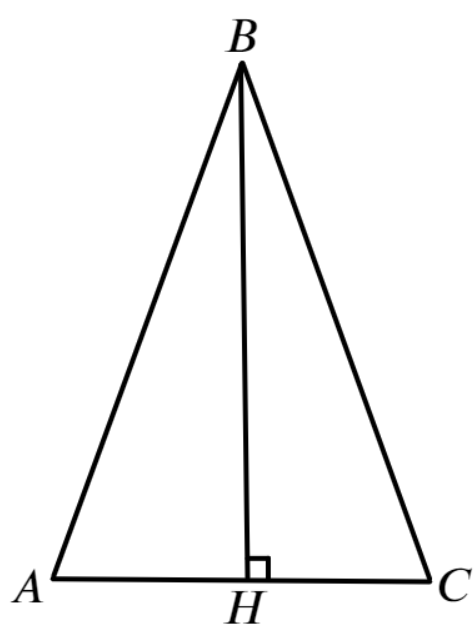
\includegraphics[scale=0.35]{g9-45.png}}
\end{figure}\\
Пусть боковая сторона треугольника равна $a,$ тогда по теореме косинусов $AC^2=a^2+a^2-2\cdot a\cdot a\cdot \cos(\angle B)=2a^2-\cfrac{10}{9}a^2=\cfrac{8}{9}a^2,$
тогда $AC=\cfrac{2\sqrt{2}}{3}a.$ Опустим из вершины высоту и медиану $BH,$ тогда $\cos(\angle A)=\cfrac{AH}{AB}=\cfrac{\cfrac{\sqrt{2}}{3}a}{a}=\cfrac{\sqrt{2}}{3},$
а $\sin(\angle A)=\sqrt{1-\cos^2(\angle A)}=\sqrt{1-\cfrac{2}{9}}=\cfrac{\sqrt{7}}{3}.$\\
